\chapter{Methodik}
\label{chap:methodik}

Für die Segmentierung der Marsoberfläche wird der Ansatz von Kanezaki \etal \cite{kanezaki_18} aus Unterabschnit~\ref{ssec:kanezaki} abgewandelt. Das Ziel besteht daraus, eine Eingabebilddatei durch neuronale Netze zu segmentieren, allerdings ohne vorhandene Ground Truth.

Zur Modifikation des genannten Algorithmus existieren viele unterschiedliche Möglichkeiten, einzelne Elemente zu ersetzen, welche in den folgenden Abschnitten beschrieben werden.

\section{Initialisierung}
\label{sec:initialisierung}

Die wohl wichtigste Veränderung des ursprünglichen Algorithmus besteht aus der Modifizierung des Initialisierungsalgorithmus.

Der von Kanezaki \etal genutzte SLIC-Algorithmus eignet sich zwar gut für die meisten mehrfarbigen Fotografien, da die Aufnahmen der Marsoberfläche allerdings nur in Graustufen vorhanden sind, würden so hier keine guten Ergebnisse produziert werden.

\begin{figure}[h!]
	\centering
	\begin{subfigure}[t]{0.32\textwidth}
		\centering
		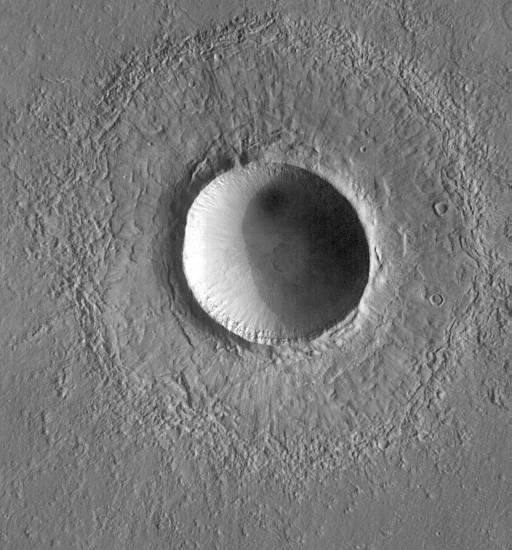
\includegraphics[width=\textwidth,keepaspectratio]{images/Gre13_01.jpg}
		\captionsetup{format=plain,width=0.85\textwidth}
		\caption{Eingabebild, aus \cite[Kap.~7]{greeley_13}}
		\label{fig:slic_vs_tsugf_in}
	\end{subfigure}
	\hfill
	\begin{subfigure}[t]{0.32\textwidth}
		\centering
		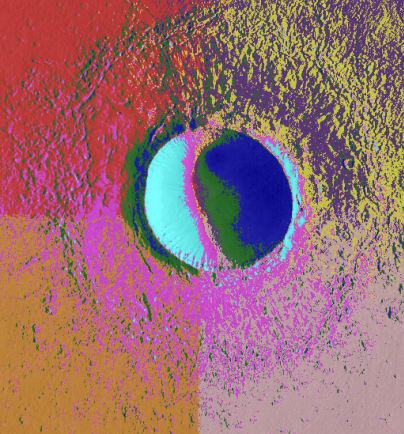
\includegraphics[width=\textwidth,keepaspectratio]{images/gen/GEN_slic_vs_tsugf_01.png}
		\captionsetup{format=plain,width=0.85\textwidth}
		\caption{Ergebnis des SLIC-Algorithmus angewandt auf die Eingabedatei}
		\label{fig:slic_vs_tsugf_slic}
	\end{subfigure}
	\hfill
	\begin{subfigure}[t]{0.32\textwidth}
		\centering
		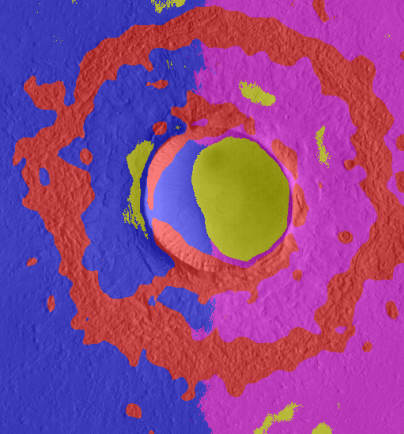
\includegraphics[width=\textwidth,keepaspectratio]{images/gen/GEN_slic_vs_tsugf_02.png}
		\captionsetup{format=plain,width=0.85\textwidth}
		\caption{Ergebnis des texturbasierten Clusterings der Eingabedatei}
		\label{fig:slic_vs_tsugf_tsugf}
	\end{subfigure}
	\caption{Clustering eines Graustufenbildes}
\end{figure}

So ergibt ein Clustering des Kraters aus Unterabschnitt~\ref{ssec:mars_surface} durch den SLIC-Algorithmus \cite{achanta_10} das in \figurename~\ref{fig:slic_vs_tsugf_slic} sichtbare Ergebnis.\footnote{SLIC-Implementierung: \texttt{scikit-image}\\Parameter: \texttt{compactness=5, n\_segments=10, enforce\_connectivity=False}} Dort ist erkennbar, dass der Krater in jeweilige Licht- und Schattenregionen (bedingt durch den Lichteinfall im flachen Winkel) unterteilt wird. Außerdem wird die raue Struktur ringförmig um den Krater herum schlecht erfasst: An dieser Stelle wird jeder Hügel separat als einerseits helle, andererseits dunkle Stelle markiert. Das Phänomen, dass ein Krater so durch eine starke Differenz an Licht- und Schattenregionen äußert wird sich im Großen und Ganzen zwar in Abschnitt~\ref{sec:craterdetection} zu nutze gemacht, ist hier allerdings ungewollt.

Wenn nun der in Unterabschnitt~\ref{ssec:kanezaki} beschriebene Ansatz verfolgt wird, wird das neuronale Netz daraufhin trainiert, eine Aufnahme anhand ihrer Helligkeitsinformationen hin zu trainieren. Da dies nicht gewollt ist, wird statt einem farb-/helligkeitsbasierten Clusteringalgorithmus wie SLIC ein texturbasiertes Clustering genutzt.

Statt des SLIC-Clusterings wird nun die in Unterabschnitt~\ref{ssec:tsugf} vorgestellte Methode des texturbasierten Clusterings genutzt. Das Ergebnis eines Clusterings durch diese Methode\footnote{Kombiniert mit der Filterbank aus \cite{jain_91}} ist in \figurename~\ref{fig:slic_vs_tsugf_tsugf} sichtbar: Man erkennt, dass der \enquote{Ring} um den eigentlichen Einschlagskrater eine eigenständige Textur besitzt, welche unterschiedlich zu dem Rest der Oberfläche ist. Eine ähnliche Oberflächenstruktur ist direkt um den Krater herum vorhanden. Beide Vorkommnisse dieser ähnlichen Struktur werden vom texturbasierten Clustering erfasst, in ein Segment aufgeteilt und (hier durch eine rote Färbung) markiert.

\subsection{Filterbänke}

Nun stellt sich die Frage, welche der vorgestellten Filterbänke sich gut eignet, die Eingabedatei zu clustern. Die größten Unterschiede zwischen den einzelnen Filterbänken besteht daraus, dass einige von ihnen rotationsinvariante Filter enthalten, und einige in mehreren Größen vorhanden sind. Die Größendifferenz lässt sich zwar in der Anwendung des Algorithmus ausgleichen, die Rotationsinvarianz allerdings nicht. In \figurename~\ref{fig:filterbank_comparision} ist die Anwendung der in Unterabschnitt~\ref{ssec:tsugf} vorgestellten Filterbänke auf vier Beispielbilder (\vgl Abschnitt~\ref{ssec:mars_surface}) sichtbar.

\paragraph{Krater}
Neben dem eigentlichen Krater ist auf dieser Aufnahme der Ring aus gröberem Gestein signifikant. Dieser wird von allen Filterbänken zuverlässig erkannt, wenn auch mit einer unterschiedlichen Dicke: Die LM- und S-Filterbank selektieren dieses Gestein eher großzügig, die MR-Filterbank hingegen zeigt sehr enge Markierungen dieser Region.

Alle Filterbänke formen einen Ring (oder dessen Ansatz) auf dem Kraterrand, die Maximum Response-Filterbank erzeugt zwei konzentrische Ringe

Der Krater selbst wird von den Filterkombinationen nach \cite{jain_91} und der LM-Filterbank leider nur in Hell- und Dunkel-Regionen aufgeteilt, die S-Filterbank zeigt innerhalb des Kraters kein brauchbares Ergebnis. Eine Ausnahme stellt die Maximum-Response-Filterbank dar, welche neben den zwei erwähnten konzentrischen Clustern den Bereich innerhalb des Kraters als ein einziges Cluster erkennt. Die Maximum Response-Bank erzeugt in diesem Bereich das Ergebnis, welches sich wohl als bestes zur Weiterverarbeitung eignet.

\paragraph{Vulkan}
Der Vulkanberg wird leider von keiner Filterbank optimal erkannt. Der äußere Rand wird nur von der S-Filterbank als ein Cluster erkannt, dies allerdings nicht sehr genau. Der rauere Bereich der Oberfläche, was kleinere Krater miteinbeschließt, wird vom MR-Filter am ehesten und genausten erkannt (in violett markiert), auf dem zweiten Platz folgt die Filterbank nach \cite{jain_91}, welche zwar alle Krater in ein Cluster fügt (violett), allerdings eher gröber.

Die Vulkanmitte wird von keiner Filterbank erkannt, nur bei der MR-Bank lässt sich eine ringförmige, rauere Stelle um den Krater herum erahnen. Außerdem ist interessant, dass der LM-Filter die Bergspitzen in vom Umfeld getrennte Cluster einteilt (blau und violett). Somit scheint es, als liese sich diese Aufnahme über keine Filterbank gut clustern, am ehesten eignet sich allerdings erneut die MR-Bank.

\paragraph{Vulkan mit strahlenförmigen Merkmalen}

Das Ziel bei der Nutzung dieser Marsaufnahme zur Analyse besteht daraus zu analysieren, mit welcher Filterbank die konzentrischen Strahlen am genauesten erkannt werden. Des Weiteren existieren auf der Aufnahme noch Krater, welche es separat zu clustern gilt.

Die Filterbank nach \cite{jain_91} erkennt die gröberen Strukturen (Strahlen und Krater), fügt diese allerdings in dasselbe Cluster ein (gelb und rot).

Die LM-Filterbank scheint kein brauchbares Ergebnis zu produzieren, sie erkennt im Allgemeinen nur einige der Krater (gelb) separat von deren Umfeld, die Strahlen sind nicht geeignet geclustert worden.

Die Schmid-Filterbank clustert einen Großteil der Strahle gemeinsam in ein Cluster (rot). Die Krater hingegen sind nicht fest einer Clusterart zugewiesen.

Wie in den vorherigen Test ist das Ergebnis der MR-Filterbank schon fast zu genau, die Cluster sind sehr fein gehalten. Im Gegensatz zu den Alternativen, werden hier die Krater relativ zuverlässig in gelbe Cluster eingeordnet, die Strahlen sind leider zu fein, als das sie getrennt erkennbar sind. Dieses Phänomen könnte sich allerdings in der praktischen Anwendung zunutze gemacht werden, da dafür eine zu feine Initialisierung notwendig ist.

\paragraph{Gletscher}

Der Gletscher ist subjektiv betrachtet das schwierigste der hier vorgestellten Probleme, da er an vielen seiner Ränder keine feste Grenze zu benachbarten Regionen zeigt, nur links auf der Aufnahme ist er durch eine Hügelreihe strikt begrenzt. Diese Grenze wird von allen Filterbänken in ein getrenntes Cluster unterteilt,mit Ausnahme der Filterbank nach \cite{jain_91}: Diese produziert kein geeignetes Ergebnis, nur die stärker erkennbaren \enquote{Streifen} werden gut erkannt (blau). Die LM-Filterbank erkennt zwar die Abgrenzung auf der linken Seite, allerdings keine anderen Regionen korrekt. Sie liefert bei diesem Bild das wohl schlechteste Ergebnis. Die Maximum-Response Methode und die Filterbank nach \cite{leung_01} liefern zwar etwas bessere Ergebnisse, diese sind allerdings nicht gut. Die MR-Bank erzeugt erneut sehr feine Cluster.

\paragraph{}
Zusammengefasst erzeugt aus dieser Auswahl an Filterbänden die Maximum Response-Methode von \cite{visgeo} das wohl am ehesten geeignete Ergebnis zur Weiterverarbeitung. Auf zweitem Platz folgt die Schmid-Filterbank.

\begin{figure}[h!]
\begin{tabular}{p{0.2\textwidth}p{0.2\textwidth}p{0.2\textwidth}p{0.2\textwidth}p{0.2\textwidth}}
	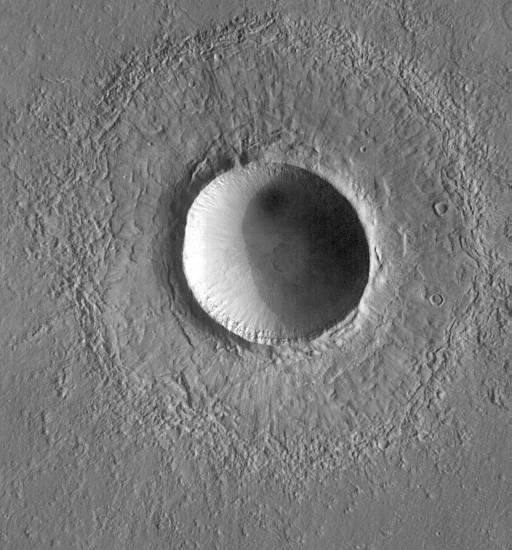
\includegraphics[width=0.2\textwidth]{images/Gre13_01.jpg} &
	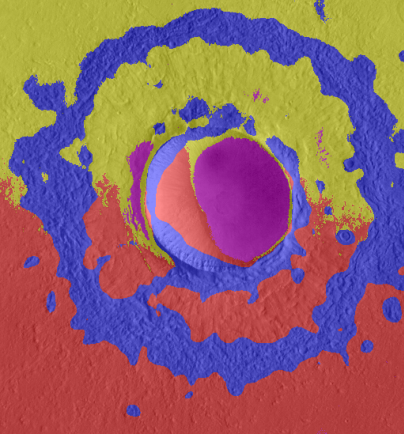
\includegraphics[width=0.2\textwidth]{images/gen/GEN_filterbanks_Gre13_01_TSUGF.png} &
	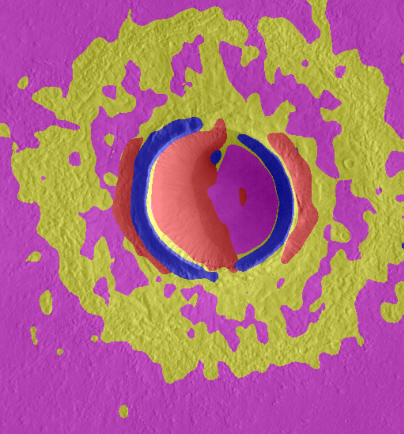
\includegraphics[width=0.2\textwidth]{images/gen/GEN_filterbanks_Gre13_01_LM.png} &
	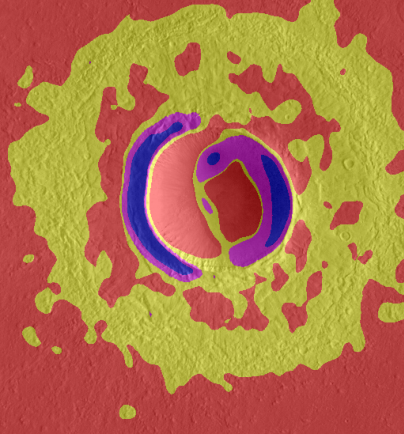
\includegraphics[width=0.2\textwidth]{images/gen/GEN_filterbanks_Gre13_01_S.png} &
	\includegraphics[width=0.2\textwidth]{images/gen/GEN_filterbanks_Gre13_01_MR.png} \\
	
	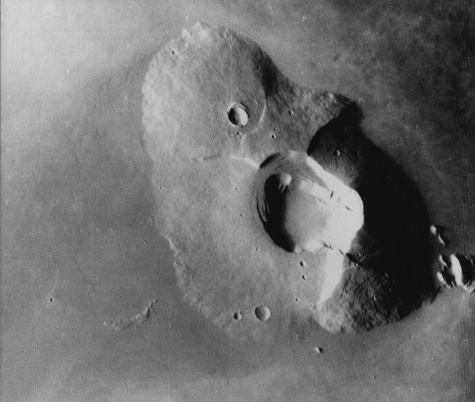
\includegraphics[width=0.2\textwidth]{images/Gre13_02.jpg} &
	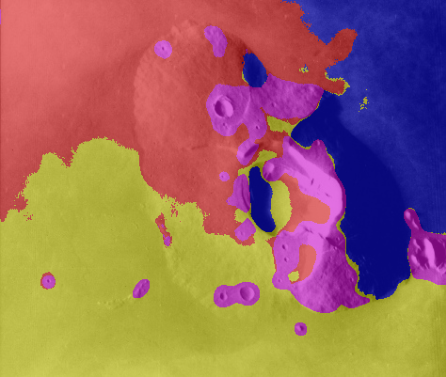
\includegraphics[width=0.2\textwidth]{images/gen/GEN_filterbanks_Gre13_02_TSUGF.png} &
	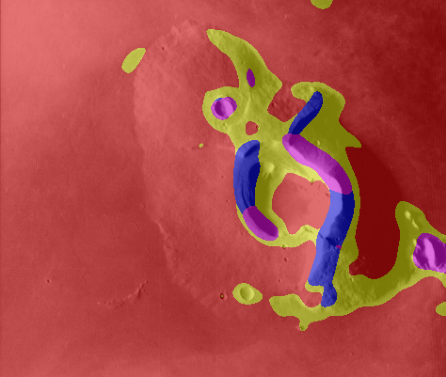
\includegraphics[width=0.2\textwidth]{images/gen/GEN_filterbanks_Gre13_02_LM.png} &
	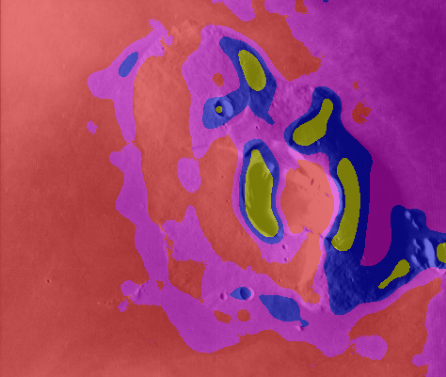
\includegraphics[width=0.2\textwidth]{images/gen/GEN_filterbanks_Gre13_02_S.png} &
	\includegraphics[width=0.2\textwidth]{images/gen/GEN_filterbanks_Gre13_02_MR.png} \\
	
	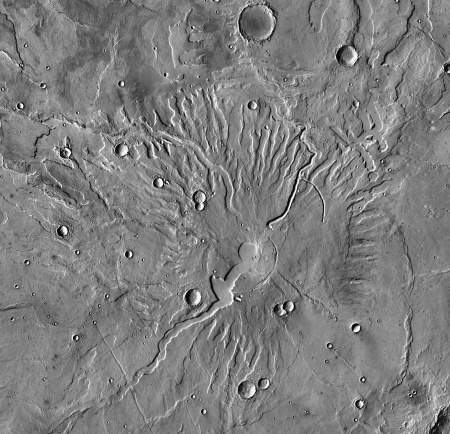
\includegraphics[width=0.2\textwidth]{images/Gre13_03.jpg} &
	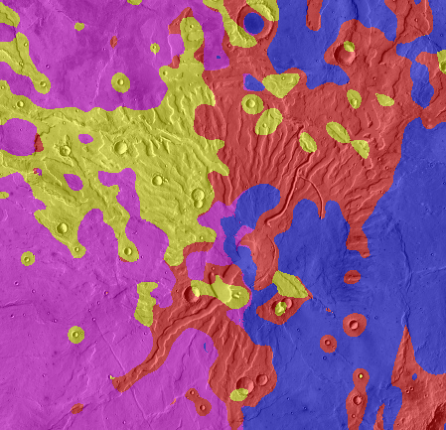
\includegraphics[width=0.2\textwidth]{images/gen/GEN_filterbanks_Gre13_03_TSUGF.png} &
	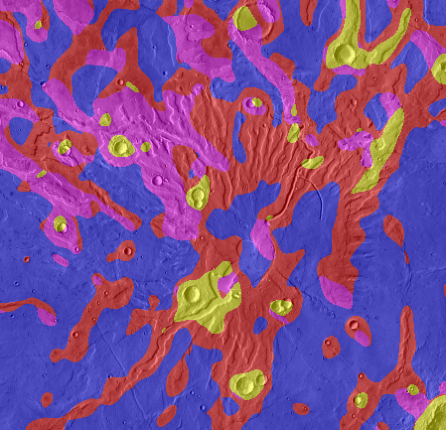
\includegraphics[width=0.2\textwidth]{images/gen/GEN_filterbanks_Gre13_03_LM.png} &
	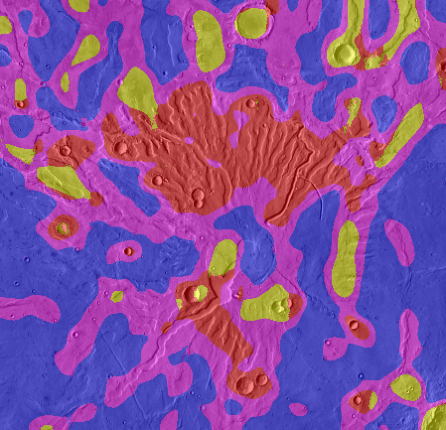
\includegraphics[width=0.2\textwidth]{images/gen/GEN_filterbanks_Gre13_03_S.png} &
	\includegraphics[width=0.2\textwidth]{images/gen/GEN_filterbanks_Gre13_03_MR.png} \\
	
	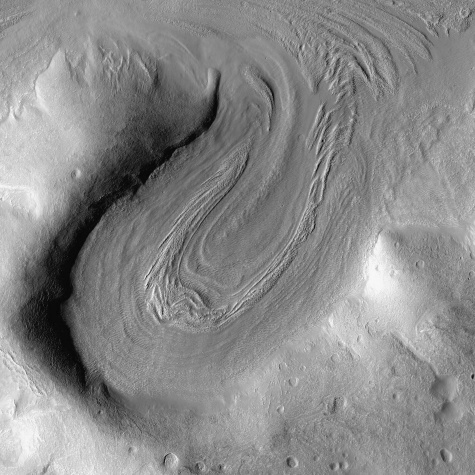
\includegraphics[width=0.2\textwidth]{images/Gre13_05.jpg} &
	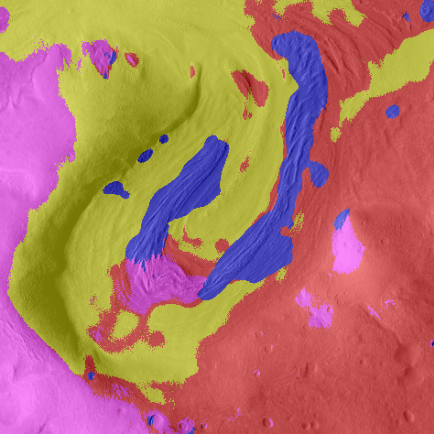
\includegraphics[width=0.2\textwidth]{images/gen/GEN_filterbanks_Gre13_05_TSUGF.png} &
	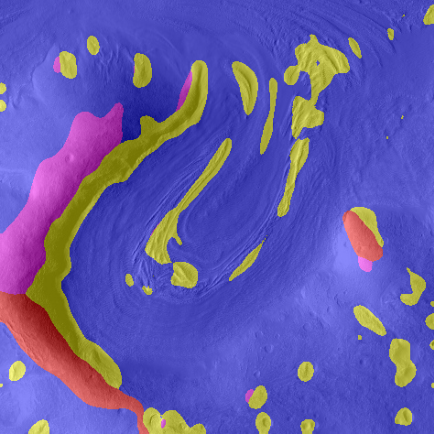
\includegraphics[width=0.2\textwidth]{images/gen/GEN_filterbanks_Gre13_05_LM.png} &
	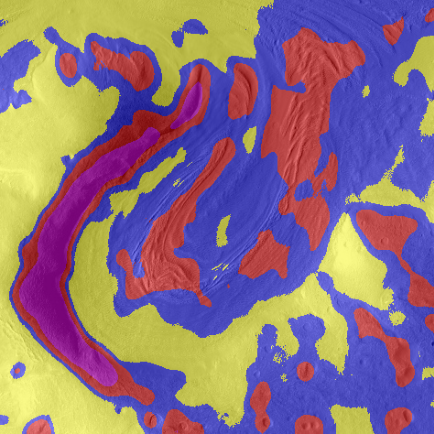
\includegraphics[width=0.2\textwidth]{images/gen/GEN_filterbanks_Gre13_05_S.png} &
	\includegraphics[width=0.2\textwidth]{images/gen/GEN_filterbanks_Gre13_05_MR.png} \\
	
	\centering Eingabe, aus \cite{greeley_13} &
	\centering Filterbank nach \cite{jain_91} &
	\centering LM-Filterbank \cite{leung_01} &
	\centering S-Filterbank \cite{schmid_01} &
	\centering MR-Filterbank \cite{visgeo} \\
\end{tabular}
\caption{Vergleich verschiedener Filterbänke auf Bildern der Marsoberfläche (Krater, Vulkan, Vulkan mit strahlenförmigen Merkmalen, Gletscher). Die Farben der jeweilgen Cluster wurden zufällig gewählt und sagen nichts über deren Inhalt aus. Alle Bilder wurden in vier Cluster eingeteilt.}
\label{fig:filterbank_comparision}
\end{figure}

\subsection{Größe und Gewichtungen}

Neben der Auswahl einer geeigneten Filterbank lassen sich in dieser noch die einzelnen Gewichtungen anpassen: So könnten \zB die Gewichtung der Koordinaten der Pixel zueinander oder die Relevanz von ähnlichen Farbwertden modifiziert werden.

\section{Netzwerkarchitektur}

Die Netzwerkarchitektur im originalen Paper stellt ein relativ einfaches Netzwerk zur Objekterkennung oder Bildsegmentierung dar:



\section{Abbruchkriterium}

\section{Preprocessing}

\section{Anpassungen für mehrfarbige Fotografien}